\chapter{रासायनिक बलगतिकी: दर नियम}\label{ch:b1:rate-laws}

दूध फ़्रिज में एक सप्ताह टिकता है और गर्मी में खुली मेज़ पर एक दिन। किसी दवा के
डिब्बे पर लिखा होता है ``\qty{25}{\celsius} से नीचे रखें'' और उस पर दो-तीन वर्ष आगे की
समाप्ति-तिथि होती है, जिसे निर्माता के पास सीधे देखने का समय नहीं था।
साम्य स्थिरांक बताते हैं कि कोई अभिक्रिया कहाँ समाप्त होती है; वहाँ तक पहुँचने में
कितना समय लगता है, इस बारे में वे कुछ नहीं बताते। यह रासायनिक बलगतिकी का
क्षेत्र है। यह अध्याय अभिक्रिया की दर को परिभाषित करता है, वे \omterm{def:b1:rate-laws:order}{दर
नियम} जो उसे सांद्रताओं के रूप में व्यक्त करते हैं, वे समाकलित रूप
जो किसी भी समय की सांद्रताओं का पूर्वानुमान देते हैं, वे प्रायोगिक विधियाँ जिनसे
\omterm{def:b1:rate-laws:order}{दर नियम} निर्धारित होता है, और \omterm{thm:b1:rate-laws:arrhenius}{आरेनियस नियम} जो ताप के प्रभाव का वर्णन करता है
--- वह साधन जिससे कुछ सप्ताहों के प्रयोगों में किसी दवा की भंडारण-आयु का
पूर्वानुमान लगाया जाता है।

\begin{recall}
पुस्तक 1 (कक्षा 12) ने किसी स्पीशीज़ की प्रकटन और \omterm{def:b1:rate-laws:rate}{लोप दर},
गतिक कारकों (सांद्रता, ताप, उत्प्रेरक) और
प्रथम कोटि की अभिक्रिया की \omterm{def:b1:rate-laws:half-life}{अर्ध-आयु} का परिचय दिया था। \omterm{def:b1:extent-q-and-k:extent}{अभिक्रिया की प्रगति} $\xi$
की परिभाषा \cref{def:b1:extent-q-and-k:extent} में दी गई।
\end{recall}

\begin{omfigure}
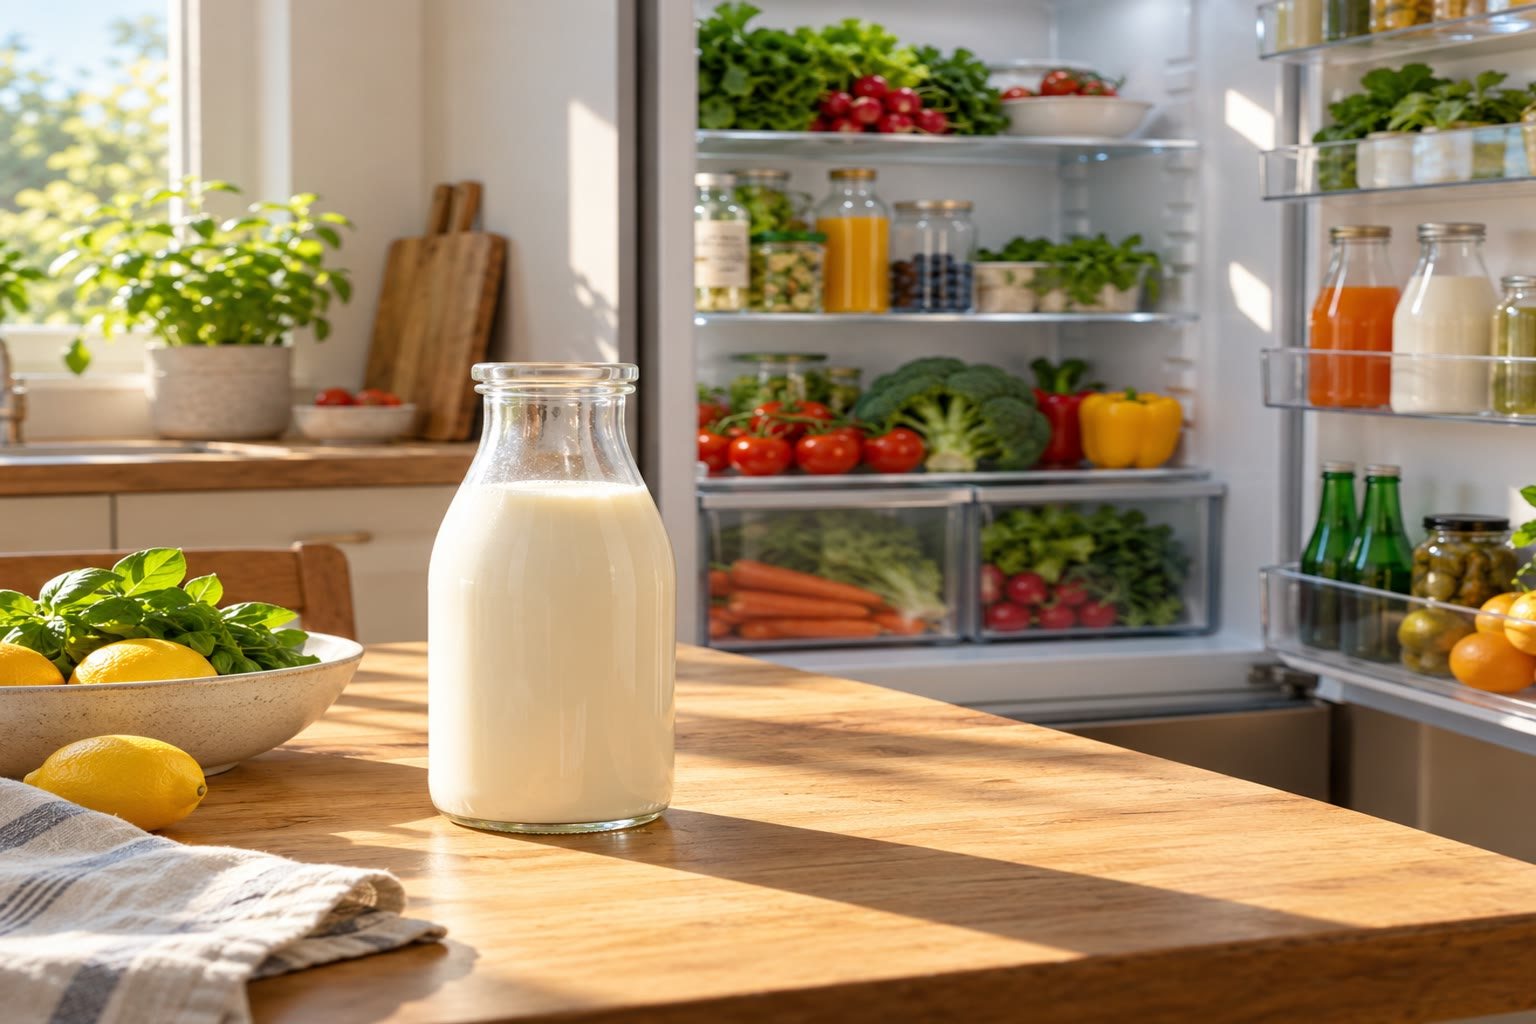
\includegraphics[width=0.55\linewidth]{images/book2/ai/b1-08-milk-kitchen.jpg}

{\small धूप में, खुले फ़्रिज के पास छोड़ी गई दूध की बोतल।
उसे ख़राब करने वाली अभिक्रियाएँ गर्मी के ताप पर ठंड की तुलना में कई गुना तेज़
चलती हैं।}
\end{omfigure}

\section{अभिक्रिया की दर}

\begin{definition}[अभिक्रिया दर, निर्माण और लोप की दरें]\label{def:b1:rate-laws:rate}
अभिक्रिया $0 = \sum_i \nu_i\mathrm{A}_i$ के लिए, जो स्थिर आयतन $V$ वाले बंद
रिएक्टर में होती है, \emph{अभिक्रिया दर}\index{अभिक्रिया दर}
है
\[
  v = \frac{1}{V}\frac{\dd\xi}{\dd t} = \frac{1}{\nu_i}\frac{\dd[\mathrm{A}_i]}{\dd t}
  \quad\text{(कोई भी } i\text{)},
\]
\unit{mol.L^{-1}.s^{-1}} में। किसी उत्पाद की \emph{निर्माण दर}\index{निर्माण दर}
$\dd[\mathrm{A}_i]/\dd t$ है; किसी अभिकारक की \emph{लोप
दर}\index{लोप दर}
$-\dd[\mathrm{A}_i]/\dd t$ है।
\end{definition}

\begin{proposition}[सभी स्पीशीज़ के लिए एक ही दर]\label{prop:b1:rate-laws:rate-relations}
\omterm{def:b1:rate-laws:rate}{अभिक्रिया दर} इस पर निर्भर नहीं करती कि उसका अनुसरण करने के लिए कौन-सी स्पीशीज़ चुनी गई:
$a\,\mathrm{A} + b\,\mathrm{B} \longrightarrow c\,\mathrm{C} + d\,\mathrm{D}$ के लिए,
\[
  v = -\frac1a\frac{\dd[\ce{A}]}{\dd t} = -\frac1b\frac{\dd[\ce{B}]}{\dd t}
  = \frac1c\frac{\dd[\ce{C}]}{\dd t} = \frac1d\frac{\dd[\ce{D}]}{\dd t} .
\]
\end{proposition}

\begin{proof}
$[\mathrm{A}_i] = (n_{i,0} + \nu_i\xi)/V$, जहाँ $V$ स्थिर है, इसलिए
$\dd[\mathrm{A}_i]/\dd t = (\nu_i/V)\,\dd\xi/\dd t = \nu_i v$।
\end{proof}

\begin{example}[डाइनाइट्रोजन पेंटॉक्साइड का विघटन]\label{ex:b1:rate-laws:n2o5}
\ce{2N2O5 -> 4NO2 + O2} के लिए: $v = -\frac12\frac{\dd[\ce{N2O5}]}{\dd t} =
\frac14\frac{\dd[\ce{NO2}]}{\dd t} = \frac{\dd[\ce{O2}]}{\dd t}$। नाइट्रोजन
डाइऑक्साइड डाइऑक्सीजन से चार गुना तेज़ी से प्रकट होती है, और डाइनाइट्रोजन पेंटॉक्साइड
उससे दोगुनी तेज़ी से लुप्त होती है जितनी तेज़ी से डाइऑक्सीजन प्रकट होती है।
\end{example}

\section{दर नियम और कोटियाँ}

\begin{definition}[दर नियम, कोटियाँ, दर स्थिरांक]\label{def:b1:rate-laws:order}
\emph{दर नियम}\index{दर नियम} दर को
सांद्रताओं के फलन के रूप में व्यक्त करता है। कोई अभिक्रिया \emph{कोटि रखती है} जब उसका दर नियम
इस रूप का हो
\[
  v = k\,[\mathrm{A}]^{p}\,[\mathrm{B}]^{q} \cdots ;
\]
जहाँ घातांक $p$, $q$, \dots\ A, B, \dots\ के सापेक्ष \emph{आंशिक कोटियाँ}\index{आंशिक कोटि}
हैं, उनका योग \emph{समग्र
कोटि}\index{समग्र कोटि} है, और $k$ \emph{दर स्थिरांक}\index{दर स्थिरांक} है,
जो केवल ताप पर निर्भर करता है। कोटियाँ
प्रयोग से ज्ञात की जाती हैं; उनका रससमीकरणमितीय गुणांकों के बराबर होना आवश्यक नहीं, और वे
भिन्नात्मक या शून्य भी हो सकती हैं।
\end{definition}

\begin{remark}[$k$ के मात्रक]\label{rem:b1:rate-laws:units}
चूँकि $v$, \unit{mol.L^{-1}.s^{-1}} में है, इसलिए $k$ कोटि 0 के लिए
\unit{mol.L^{-1}.s^{-1}} में, कोटि 1 के लिए \unit{s^{-1}} में,
कोटि 2 के लिए \unit{L.mol^{-1}.s^{-1}} में, और व्यापक रूप में
$(\unit{mol/L})^{1-n}\,\unit{s^{-1}}$ में होता है, \omterm{def:b1:rate-laws:order}{समग्र कोटि} $n$ के लिए। $k$ का
मात्रक \omterm{def:b1:rate-laws:order}{समग्र कोटि} बता देता है।
\end{remark}

\begin{remark}[कोटि-रहित अभिक्रियाएँ]\label{rem:b1:rate-laws:no-order}
हर अभिक्रिया की कोई कोटि नहीं होती। कुछ अभिक्रियाओं की दर ऐसा भिन्न होती है
जिसके हर में सांद्रताएँ होती हैं, या वह किसी उत्पाद की
सांद्रता पर निर्भर करती है। ऐसे \omterm{def:b1:rate-laws:order}{दर नियमों} की व्याख्या अभिक्रिया की
क्रियाविधि से होती है (\cref{ch:b1:elementary-steps})। कोई अभिक्रिया
केवल आरंभ में भी कोटि रख सकती है: \omterm{def:b1:rate-laws:initial-rate}{प्रारंभिक दर} नियम।
\end{remark}

\section{समाकलित दर नियम और अर्ध-आयु}

\begin{definition}[अर्ध-आयु]\label{def:b1:rate-laws:half-life}
किसी अभिकारक की \emph{अर्ध-आयु}\index{अर्ध-आयु} $t_{1/2}$ वह समय है
जिसके बाद उसकी प्रारंभिक मात्रा का आधा भाग खप चुका होता है।
\end{definition}

\begin{theorem}[समाकलित दर नियम]\label{thm:b1:rate-laws:integrated}
अभिक्रिया $a\mathrm{A} \rightarrow \text{उत्पाद}$ के लिए, जिसकी दर $v = -\frac1a\frac{\dd[\ce{A}]}
{\dd t} = k[\ce{A}]^n$ है, और $[\ce{A}](0) = a_0$ के साथ:
\begin{center}
\begin{tabular}{llll}
\hline
कोटि & समाकलित नियम & रैखिक आलेख & \omterm{def:b1:rate-laws:half-life}{अर्ध-आयु} \\
\hline
0 & $[\ce{A}] = a_0 - akt$ & $[\ce{A}]$ बनाम $t$ & $a_0/(2ak)$ \\
1 & $[\ce{A}] = a_0\,\eu^{-akt}$ & $\ln[\ce{A}]$ बनाम $t$ & $\ln2/(ak)$ \\
2 & $\dfrac{1}{[\ce{A}]} = \dfrac{1}{a_0} + akt$ & $1/[\ce{A}]$ बनाम $t$ & $1/(ak\,a_0)$ \\
\hline
\end{tabular}
\end{center}
\end{theorem}

\begin{proof}
$c = [\ce{A}]$ लिखिए, तब $\dd c/\dd t = -akc^n$।
\emph{कोटि 0}: $\dd c/\dd t = -ak$, अतः $c = a_0 - akt$ (जब तक
$c = 0$ न हो, तब तक मान्य)। \emph{कोटि 1}: $\dd c/\dd t = -akc$ एक प्रथम कोटि का रैखिक
अवकल समीकरण है जिसका हल $c = a_0\eu^{-akt}$ है।
\emph{कोटि 2}: $\dd c/c^2 = -ak\,\dd t$; 0 से $t$ तक समाकलन करने पर
$-1/c + 1/a_0 = -akt$, इसलिए $1/c = 1/a_0 + akt$। \omterm{def:b1:rate-laws:half-life}{अर्ध-आयु}: हर नियम में $c =
a_0/2$ रखकर $t$ के लिए हल कीजिए।
\end{proof}

\begin{proposition}[अर्ध-आयु परीक्षण]\label{prop:b1:rate-laws:half-life-test}
\omterm{def:b1:rate-laws:half-life}{अर्ध-आयु} प्रारंभिक सांद्रता से स्वतंत्र होती है यदि और केवल यदि
अभिक्रिया कोटि 1 की हो। कोटि 0 के लिए यह $a_0$ के समानुपाती है और
कोटि 2 के लिए $1/a_0$ के। प्रथम कोटि की अभिक्रिया हर क्रमिक \omterm{def:b1:rate-laws:half-life}{अर्ध-आयु} में
बचे हुए का आधा खोती है: $m$ \omterm{def:b1:rate-laws:half-life}{अर्ध-आयुओं} के बाद भिन्न $2^{-m}$
शेष रहता है।
\end{proposition}

\begin{proof}
कोटि $n \ne 1$ के लिए चरों को अलग करने पर $t_{1/2} = \dfrac{2^{n-1} -
1}{(n-1)\,ak\,a_0^{n-1}}$ मिलता है, जो $a_0$ पर निर्भर करता है जब तक $n = 1$ न हो;
$n = 1$ के लिए $t_{1/2} = \ln2/(ak)$। कोटि 1 के लिए $c(t + t_{1/2}) = c(t)/2$, हर $t$ पर,
क्योंकि $\eu^{-ak(t + t_{1/2})} = \eu^{-akt}/2$।
\end{proof}

\begin{omfigure}
\begin{tikzpicture}
\begin{axis}[name=p0,
  width=0.36\linewidth, height=4.6cm,
  xmin=0, xmax=60, ymin=0, ymax=1.05,
  axis x line=bottom, axis y line=left,
  xlabel={$t$ (min)}, title={कोटि 0: $[\ce{A}]$},
  title style={font=\small}, xtick={0,20,40,60},
  tick label style={font=\scriptsize}, label style={font=\small}]
\addplot[omDef, thick] table[x=t, y=A0] {figdata/out/bachelor-1-integrated-rate-laws.dat};
\end{axis}
\begin{axis}[at={(p0.east)}, anchor=west, xshift=0.9cm, name=p1,
  width=0.36\linewidth, height=4.6cm,
  xmin=0, xmax=60, ymin=-3.2, ymax=0.2,
  axis x line=bottom, axis y line=left,
  xlabel={$t$ (min)}, title={कोटि 1: $\ln[\ce{A}]$},
  title style={font=\small}, xtick={0,20,40,60},
  tick label style={font=\scriptsize}, label style={font=\small}]
\addplot[omProp, thick] table[x=t, y=lnA1] {figdata/out/bachelor-1-integrated-rate-laws.dat};
\end{axis}
\begin{axis}[at={(p1.east)}, anchor=west, xshift=0.9cm,
  width=0.36\linewidth, height=4.6cm,
  xmin=0, xmax=60, ymin=0, ymax=4.2,
  axis x line=bottom, axis y line=left,
  xlabel={$t$ (min)}, title={कोटि 2: $1/[\ce{A}]$},
  title style={font=\small}, xtick={0,20,40,60},
  tick label style={font=\scriptsize}, label style={font=\small}]
\addplot[omThm, thick] table[x=t, y=invA2] {figdata/out/bachelor-1-integrated-rate-laws.dat};
\end{axis}
\end{tikzpicture}

\begin{tikzpicture}
\begin{axis}[
  width=0.62\linewidth, height=5.0cm,
  xmin=0, xmax=60, ymin=0, ymax=1.05,
  axis x line=bottom, axis y line=left,
  xlabel={$t$ (min)}, ylabel={$[\ce{A}]$ (mol/L)}, xtick={0,10,20,30,40,50,60},
  tick label style={font=\small}, label style={font=\small},
  legend style={font=\small, draw=none, at={(0.98,0.98)}, anchor=north east}]
\addplot[omDef, thick] table[x=t, y=A0] {figdata/out/bachelor-1-integrated-rate-laws.dat};
\addplot[omProp, thick] table[x=t, y=A1] {figdata/out/bachelor-1-integrated-rate-laws.dat};
\addplot[omThm, thick] table[x=t, y=A2] {figdata/out/bachelor-1-integrated-rate-laws.dat};
\legend{कोटि 0, कोटि 1, कोटि 2}
\draw[dotted] (axis cs:0,0.5) -- (axis cs:20,0.5);
\end{axis}
\end{tikzpicture}

{\small समान प्रारंभिक सांद्रता
(\qty{1.00}{mol/L}) और समान \omterm{def:b1:rate-laws:initial-rate}{प्रारंभिक दर}
(\qty{0.050}{mol.L^{-1}.min^{-1}}) वाली तीन अभिक्रियाएँ। ऊपर: हर समाकलित नियम
अपने निर्देशांकों में सरल रेखा बन जाता है। नीचे: सांद्रताएँ;
\omterm{def:b1:rate-laws:half-life}{अर्ध-आयु} 10, 13.9 और 20 मिनट हैं।}
\end{omfigure}

\section{दर नियम ज्ञात करना}

\begin{method}[समाकल विधि]\label{met:b1:rate-laws:integral}
मापनों $[\ce{A}](t)$ से किसी कोटि की जाँच के लिए: $[\ce{A}]$,
$\ln[\ce{A}]$ और $1/[\ce{A}]$ को $t$ के सापेक्ष आलेखित कीजिए; जो आलेख सरल
रेखा हो वही कोटि देता है, और उसकी प्रवणता $k$ देती है (प्रवणता क्रमशः $-ak$, $-ak$ या $+ak$)।
\end{method}

\begin{method}[अर्ध-आयु विधि]\label{met:b1:rate-laws:half-life}
कई प्रारंभिक सांद्रताओं के लिए \omterm{def:b1:rate-laws:half-life}{अर्ध-आयु} मापिए: स्थिर हो तो
कोटि 1; $a_0$ के समानुपाती हो तो कोटि 0; $1/a_0$ के समानुपाती हो तो कोटि
2। एक ही प्रयोग में $a_0$ से $a_0/2$ तक
और $a_0/2$ से $a_0/4$ तक जाने के समयों की तुलना कीजिए: बराबर समय का अर्थ है कोटि 1।
\end{method}

\begin{definition}[प्रारंभिक दर]\label{def:b1:rate-laws:initial-rate}
\emph{प्रारंभिक दर}\index{प्रारंभिक दर} $v_0$, $t = 0$ पर दर है,
जिसे वक्र $[\ce{A}](t)$ के मूलबिंदु पर स्पर्शरेखा की प्रवणता के रूप में पढ़ा जाता है
और रससमीकरणमितीय गुणांक से भाग दिया जाता है। उस क्षण
सांद्रताएँ ज्ञात प्रारंभिक सांद्रताएँ होती हैं और कोई उत्पाद हस्तक्षेप नहीं करता।
\end{definition}

\begin{method}[प्रारंभिक दरों की विधि]\label{met:b1:rate-laws:initial-rates}
$v_0 = k[\ce{A}]_0^p[\ce{B}]_0^q$ के लिए: ऐसे प्रयोग कीजिए जिनमें केवल
$[\ce{A}]_0$ बदले; तब $\ln v_0 = \ln(k[\ce{B}]_0^q) + p\ln[\ce{A}]_0$,
और $\ln v_0$ बनाम $\ln[\ce{A}]_0$ की प्रवणता $p$ है। व्यवहार में
$[\ce{A}]_0$ को दोगुना करने से $v_0$, $2^p$ से गुणा हो जाता है। B के लिए भी यही कीजिए।
\end{method}

\begin{definition}[पृथक्करण विधि, आभासी कोटि]\label{def:b1:rate-laws:apparent-order}
\emph{पृथक्करण विधि}\index{पृथक्करण विधि} में एक को छोड़कर
सभी अभिकारक बड़े आधिक्य में (दस गुना या अधिक) रखे जाते हैं। उनकी सांद्रताएँ
व्यावहारिक रूप से स्थिर रहती हैं, और $v = k[\ce{A}]^p[\ce{B}]^q \approx k'[\ce{A}]^p$,
जहाँ $k' = k[\ce{B}]_0^q$: अभिक्रिया ऐसा व्यवहार करती है मानो उसकी
\emph{आभासी कोटि}\index{आभासी कोटि} $p$ हो और आभासी \omterm{def:b1:rate-laws:order}{दर
स्थिरांक} $k'$। इसे कोटि का ह्रास भी कहते हैं।
\end{definition}

\begin{omfigure}
\begin{tikzpicture}
\begin{axis}[
  width=0.55\linewidth, height=4.8cm,
  xmin=0, xmax=40, ymin=0, ymax=1.05,
  axis x line=bottom, axis y line=left,
  xlabel={$t$ (min)}, ylabel={$[\ce{A}]$ (mol/L)},
  xtick={0,10,20,30,40},
  tick label style={font=\small}, label style={font=\small}, clip mode=individual]
\addplot[omProp, thick] table[x=t, y=A1] {figdata/out/bachelor-1-integrated-rate-laws.dat};
\draw[omThm, thick] (axis cs:0,1) -- (axis cs:20,0);
\node[omThm, anchor=west, font=\small] at (axis cs:2,0.12) {\shortstack[r]{$t = 0$ पर\\ स्पर्शरेखा}};
\end{axis}
\end{tikzpicture}

{\small \omterm{def:b1:rate-laws:initial-rate}{प्रारंभिक दर} पढ़ना: प्रथम कोटि के वक्र के मूलबिंदु पर स्पर्शरेखा (लाल)
समय-अक्ष से $t_0 = \qty{20}{min}$ पर मिलती है, इसलिए $v_0 =
\qty{1.00}{mol/L}/\qty{20}{min} = \qty{0.050}{mol.L^{-1}.min^{-1}}$।}
\end{omfigure}

\begin{inthelab}[समय के साथ अभिक्रिया का अनुसरण]
\omterm{def:b1:rate-laws:order}{दर नियम} अभिक्रिया के चलते समय मापी गई सांद्रताओं से बनाया जाता है।
जब कोई अभिकारक या उत्पाद रंगीन हो, तो स्पेक्ट्रमप्रकाशमापी
अवशोषकता दर्ज करता है, जो उसकी सांद्रता के समानुपाती है (बीयर--लैम्बर्ट,
\cref{ch:b1:structure-spectroscopy}); जब आयन प्रकट या लुप्त होते हैं, तो
चालकतामापी चालकता का अनुसरण करता है; जब किसी बंद पात्र में गैस बनती है,
तो दाबमापी दाब का अनुसरण करता है। अन्यथा ज्ञात समयों पर नमूने लिए जाते हैं,
अभिक्रिया को ठंडा करके या तनु करके रोका (शमित किया) जाता है,
और हर नमूने का अनुमापन किया जाता है। पात्र का ताप एक तापस्थायी
कुंड द्वारा स्थिर रखा जाता है, क्योंकि $k$ उस पर प्रबल रूप से निर्भर करता है।
\end{inthelab}

\section{ताप: आरेनियस नियम}

\begin{definition}[सक्रियण ऊर्जा]\label{def:b1:rate-laws:activation-energy}
\emph{सक्रियण ऊर्जा}\index{सक्रियण ऊर्जा} $E_a$, \omterm{def:b1:rate-laws:order}{दर स्थिरांक} $k(T)$ वाली किसी
अभिक्रिया के लिए, इस प्रकार परिभाषित है:
\[
  \frac{\dd \ln k}{\dd T} = \frac{E_a}{RT^2} ,
\]
\unit{J/mol} में। जब $E_a$, $T$ से स्वतंत्र हो, तो समाकलन से
$k = A\,\eu^{-E_a/RT}$ मिलता है, जहाँ स्थिरांक $A$, जिसका मात्रक वही है जो $k$ का,
\emph{पूर्व-घातांकी गुणक}\index{पूर्व-घातांकी गुणक} है।
\end{definition}

\begin{theorem}[आरेनियस नियम]\label{thm:b1:rate-laws:arrhenius}
अधिकांश अभिक्रियाओं के लिए, ताप के सीमित परास में, \omterm{def:b1:rate-laws:order}{दर
स्थिरांक} \emph{आरेनियस नियम}\index{आरेनियस नियम} का पालन करता है
\[
  k(T) = A\,\eu^{-E_a/RT} ,
\]
जहाँ $A$ और $E_a > 0$, $T$ से स्वतंत्र हैं: $\ln k$, $1/T$ का
रैखिक फलन है, जिसकी प्रवणता $-E_a/R$ है।
\end{theorem}
\admitted

\begin{remark}[$E_a$ का अर्थ]\label{rem:b1:rate-laws:meaning}
यह नियम आनुभविक है। इसकी व्याख्या --- केवल वे आण्विक टक्करें
जो कम-से-कम $E_a$ की कोटि की ऊर्जा लेकर आती हैं, अभिक्रिया तक ले जाती हैं, और
ऐसी टक्करों का भिन्न $\eu^{-E_a/RT}$ के अनुसार बदलता है --- अगले अध्याय के
ऊर्जा प्रोफ़ाइलों के साथ रेखांकित की जाती है और तृतीय वर्ष के खंड में \omterm{def:b1:rate-laws:rate}{अभिक्रिया
दरों} के सिद्धांतों द्वारा परिमाणित की जाती है।
\end{remark}

\begin{method}[$E_a$ ज्ञात करना]\label{met:b1:rate-laws:arrhenius-plot}
कई तापों पर \omterm{def:b1:rate-laws:order}{दर स्थिरांकों} से $\ln k$ को $1/T$ के सापेक्ष आलेखित कीजिए
(केल्विन में): प्रवणता $-E_a/R$ है, अंतःखंड $\ln A$। केवल दो
तापों के साथ,
\[
  E_a = \frac{R\,\ln(k_2/k_1)}{1/T_1 - 1/T_2} .
\]
\end{method}

\begin{example}[एक मोटा नियम]\label{ex:b1:rate-laws:doubling}
$E_a = \qty{53}{kJ/mol}$ के लिए 25 से \qty{35}{\celsius} तक जाने पर
$k$, $\exp\!\big(\frac{53000}{8.314}(\frac{1}{298.15} -
\frac{1}{308.15})\big) = 2.0$ से गुणा हो जाता है। प्रचलित नियम ``दस डिग्री अधिक, दोगुनी
तेज़'' कमरे के ताप के पास उन अभिक्रियाओं के लिए लागू होता है जिनकी \omterm{def:b1:rate-laws:activation-energy}{सक्रियण ऊर्जा}
लगभग \qty{50}{kJ/mol} है; बड़े $E_a$ के लिए गुणक बड़ा होता है।
\end{example}

\begin{omfigure}
\begin{tikzpicture}
\begin{axis}[
  width=0.6\linewidth, height=5.4cm,
  xmin=2.95, xmax=3.45, ymin=-9.0, ymax=-4.2, clip mode=individual,
  axis x line=bottom, axis y line=left,
  xlabel={$1000/T$ (\unit{K^{-1}})}, ylabel={$\ln k$ ($k$, \unit{d^{-1}} में)},
  xtick={3.0,3.1,3.2,3.3,3.4}, ytick={-9,-8,-7,-6,-5},
  tick label style={font=\small}, label style={font=\small}]
\addplot[omDef, thick] table[x=invT_1e3, y=lnk] {figdata/out/bachelor-1-arrhenius-line.dat};
\addplot[only marks, mark=*, mark size=2.2pt, omThm] table[x=invT_1e3, y=lnk] {figdata/out/bachelor-1-arrhenius-points.dat};
\node[font=\small, anchor=south west] at (axis cs:3.002,-4.71) {\qty{60}{\celsius}};
\node[font=\small, anchor=south west] at (axis cs:3.095,-5.66) {\qty{50}{\celsius}};
\node[font=\small, anchor=south west] at (axis cs:3.193,-6.67) {\qty{40}{\celsius}};
\draw[dashed, black!50] (axis cs:3.354,-9.0) -- (axis cs:3.354,-8.31);
\addplot[only marks, mark=o, mark size=2.4pt, omDef] coordinates {(3.354,-8.310)};
\node[font=\small, anchor=east] at (axis cs:3.33,-8.40) {\qty{25}{\celsius}, बहिर्वेशित};
\end{axis}
\end{tikzpicture}

{\small किसी दवा के निम्नीकरण का आरेनियस आलेख (सप्ताहांत
समस्या): तीन मापे गए \omterm{def:b1:rate-laws:order}{दर स्थिरांक} (लाल) प्रवणता $-E_a/R$ वाली एक रेखा पर
पड़ते हैं; \qty{25}{\celsius} तक बहिर्वेशित करने पर यह कमरे के ताप पर
भंडारण-आयु देती है।}
\end{omfigure}

\begin{history}[आरेनियस, 1889]
स्वीडिश रसायनज्ञ स्वांते आरेनियस ने 1889 में अम्लों द्वारा सुक्रोस के प्रतीपन का
अध्ययन करते हुए प्रस्ताव रखा कि अणुओं का केवल एक छोटा भिन्न, जो
``सक्रियित'' अवस्था में हों, अभिक्रिया करता है, और यह भिन्न ताप के साथ
$\eu^{-E/RT}$ के अनुसार बढ़ता है। यह विचार, आरंभ में विवादास्पद, रासायनिक
बलगतिकी की नींव बना। आरेनियस को वैद्युत अपघटनी वियोजन के अपने सिद्धांत के लिए 1903 में
रसायन विज्ञान का नोबेल पुरस्कार मिला।
\end{history}

\begin{omfigure}
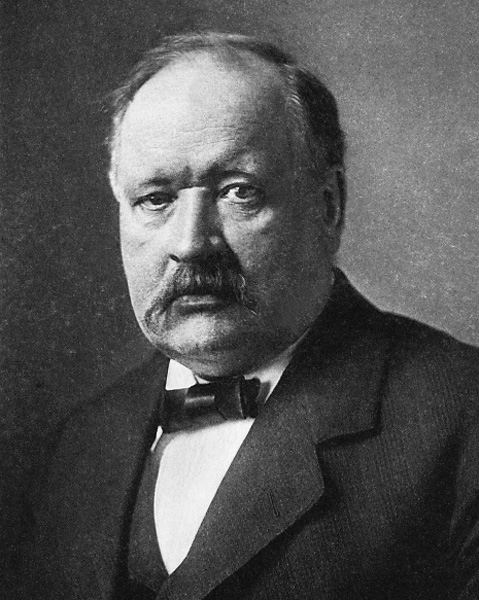
\includegraphics[width=0.22\linewidth]{images/book2/arrhenius.jpg}

{\small स्वांते आरेनियस (1859--1927), 1909 में।}
\end{omfigure}

\section{अभ्यास}

\begin{exercise}[$\star$]\label{exo:b1:rate-laws:1}
स्थिर आयतन पर \ce{2N2O5 -> 4NO2 + O2} के लिए नाइट्रोजन डाइऑक्साइड
$\qty{2.0e-4}{mol.L^{-1}.s^{-1}}$ की दर से प्रकट होती है। \omterm{def:b1:rate-laws:rate}{अभिक्रिया दर}, डाइऑक्सीजन की
\omterm{def:b1:rate-laws:rate}{निर्माण दर} और \ce{N2O5} की \omterm{def:b1:rate-laws:rate}{लोप दर} बताइए।
\end{exercise}

\begin{exercise}[$\star$]\label{exo:b1:rate-laws:2}
\omterm{def:b1:rate-laws:order}{समग्र कोटियों} 0, 1, 2 और 3 के लिए \omterm{def:b1:rate-laws:order}{दर स्थिरांक} का मात्रक बताइए,
सांद्रताएँ \unit{mol/L} में और समय सेकंड में लेकर।
\end{exercise}

\begin{exercise}[$\star$]\label{exo:b1:rate-laws:3}
प्रथम कोटि की अभिक्रिया $\mathrm{A} \longrightarrow \mathrm{B}$ के लिए $k = \qty{3.0e-3}{s^{-1}}$। उसकी
\omterm{def:b1:rate-laws:half-life}{अर्ध-आयु} और \qty{10}{min} के बाद बचे \ce{A} का भिन्न परिकलित कीजिए।
\end{exercise}

\begin{exercise}[$\star$]\label{exo:b1:rate-laws:4}
जब किसी अभिकारक की प्रारंभिक सांद्रता आधी की जाती है, तो उसकी \omterm{def:b1:rate-laws:half-life}{अर्ध-आयु}
दोगुनी हो जाती है। कोटि क्या है? यदि \omterm{def:b1:rate-laws:half-life}{अर्ध-आयु} आधी हो जाए तो?
\end{exercise}

\begin{exercise}[$\star\star$]\label{exo:b1:rate-laws:5}
किसी अभिकारक \ce{A} ($\mathrm{A} \longrightarrow \mathrm{P}$) की सांद्रता मापी जाती है: $t
= 0$, 10, 20, 30 और \qty{40}{min} पर $[\ce{A}] = 0.100$, 0.0741, 0.0549,
0.0407 और \qty{0.0301}{mol/L}। कोटि और \omterm{def:b1:rate-laws:order}{दर
स्थिरांक} ज्ञात कीजिए।
\end{exercise}

\begin{exercise}[$\star\star$]\label{exo:b1:rate-laws:6}
$\mathrm{A} + \mathrm{B} \longrightarrow \mathrm{P}$ के लिए $v_0 = \qty{2.0e-6}{mol.L^{-1}.s^{-1}}$ है जब $[\ce{A}]_0
= [\ce{B}]_0 = \qty{0.010}{mol/L}$; \qty{8.0e-6}{} जब $[\ce{A}]_0$
दोगुना किया जाए; \qty{4.0e-6}{} जब $[\ce{B}]_0$ दोगुना किया जाए। \omterm{def:b1:rate-laws:order}{आंशिक
कोटियाँ}, \omterm{def:b1:rate-laws:order}{दर नियम} और \omterm{def:b1:rate-laws:order}{दर स्थिरांक} ज्ञात कीजिए।
\end{exercise}

\begin{exercise}[$\star\star$]\label{exo:b1:rate-laws:7}
$\mathrm{A} + \mathrm{B} \longrightarrow \mathrm{P}$ का \omterm{def:b1:rate-laws:order}{दर नियम} $v = k[\ce{A}][\ce{B}]$ है।
$[\ce{B}]_0 = \qty{0.50}{mol/L}$ और $[\ce{A}]_0 = \qty{5.0e-3}{mol/L}$ के साथ
\ce{A} प्रथम कोटि की बलगतिकी से लुप्त होता है, आभासी स्थिरांक
\qty{0.012}{s^{-1}} के साथ। समझाइए और $k$ परिकलित कीजिए।
\end{exercise}

\begin{exercise}[$\star\star$]\label{exo:b1:rate-laws:8}
कोई \omterm{def:b1:rate-laws:order}{दर स्थिरांक} \qty{300}{K} पर \qty{1.0e-3}{s^{-1}} है और
\qty{320}{K} पर \qty{5.0e-3}{s^{-1}}। \omterm{def:b1:rate-laws:activation-energy}{सक्रियण ऊर्जा} और
\qty{310}{K} पर \omterm{def:b1:rate-laws:order}{दर स्थिरांक} परिकलित कीजिए।
\end{exercise}

\begin{exercise}[$\star\star$]\label{exo:b1:rate-laws:9}
अभिक्रिया $2\,\mathrm{A} \longrightarrow \mathrm{P}$ का \omterm{def:b1:rate-laws:order}{दर नियम} $v = -\frac12\frac{\dd[\ce{A}]}
{\dd t} = k[\ce{A}]^2$ है, जहाँ $k = \qty{0.50}{L.mol^{-1}.s^{-1}}$।
$[\ce{A}]_0 = \qty{0.020}{mol/L}$ से आरंभ करके \omterm{def:b1:rate-laws:half-life}{अर्ध-आयु} और
\qty{100}{s} के बाद की सांद्रता परिकलित कीजिए।
\end{exercise}

\begin{exercise}[$\star\star\star$]\label{exo:b1:rate-laws:10}
प्रथम कोटि की अभिक्रिया के लिए दिखाइए कि अभिकारक का भिन्न $f$ खपाने के लिए
आवश्यक समय $t_f = -\ln(1 - f)/(ak)$ है। 50\,\%, 75\,\%, 90\,\% और 99.9\,\% के
समयों की तुलना \omterm{def:b1:rate-laws:half-life}{अर्ध-आयुओं} में कीजिए।
\end{exercise}

\begin{exercise}[$\star\star\star$]\label{exo:b1:rate-laws:11}
एक त्वचा-पैच तब तक \qty{0.40}{mg/h} की स्थिर दर से दवा छोड़ता है
जब तक उसका भंडार, जो आरंभ में \qty{10}{mg} है, ख़ाली न हो जाए। बची हुई मात्रा का नियम लिखिए,
उसकी कोटि, \omterm{def:b1:rate-laws:half-life}{अर्ध-आयु} और वह समय बताइए जिसके बाद पैच
समाप्त हो जाता है। शून्य कोटि की बलगतिकी दवा-पैच के लिए उपयुक्त क्यों है?
\end{exercise}

\begin{exercise}[$\star\star\star$]\label{exo:b1:rate-laws:12}
दिखाइए कि \qty{298.15}{K} और \qty{308.15}{K} के बीच नियम ``दस डिग्री अधिक, दोगुनी
तेज़'' $E_a \approx
\qty{53}{kJ/mol}$ के संगत है। यही \omterm{def:b1:rate-laws:activation-energy}{सक्रियण ऊर्जा}
\qty{0}{\celsius} और \qty{10}{\celsius} के बीच कौन-सा गुणक देती है?
\end{exercise}

\section{समस्या: किसी दवा की भंडारण-आयु}

\begin{problem}[{सप्ताहांत समस्या --- एक त्वरित स्थायित्व परीक्षण:
60\,\textdegree C पर प्रथम कोटि का निम्नीकरण, तीन ताप,
आरेनियस आलेख, और कमरे के ताप पर भंडारण-आयु}]
\label{pb:b1:rate-laws:1}
किसी गोली की भंडारण-आयु $t_{90}$ (वह समय जिसके बाद सक्रिय घटक का 10\,\%
निम्नीकृत हो चुका हो) का पूर्वानुमान लगाने के लिए एक प्रयोगशाला नमूनों को
ऊँचे ताप पर रखती है और बचे हुए घटक का प्रतिशत मापती है।
\qty{60}{\celsius} पर:
\begin{center}
\begin{tabular}{lccccc}
\hline
समय (दिन) & 0 & 10 & 20 & 30 & 40 \\
शेष घटक (\%) & 100.0 & 91.4 & 83.5 & 76.3 & 69.8 \\
\hline
\end{tabular}
\end{center}
40 और \qty{50}{\celsius} पर प्राप्त \omterm{def:b1:rate-laws:order}{दर स्थिरांक}
\qty{1.27e-3}{d^{-1}} और \qty{3.48e-3}{d^{-1}} हैं। $R =
\qty{8.314}{J/(mol.K)}$ और एक माह $= \qty{30.4}{d}$ लीजिए।

\medskip
\noindent\textbf{भाग I --- 60\,\textdegree C पर कोटि।}
\begin{enumerate}
  \item हर 10-दिवसीय अंतराल में हुई हानि परिकलित कीजिए। क्या अभिक्रिया
        कोटि 0 की है?
  \item हर समय पर $\ln(\%\text{ शेष})$ परिकलित कीजिए। आप क्या निष्कर्ष निकालते हैं?
  \item \omterm{def:b1:rate-laws:order}{दर स्थिरांक} $k_{60}$ निकालिए।
  \item \qty{60}{\celsius} पर \omterm{def:b1:rate-laws:half-life}{अर्ध-आयु} परिकलित कीजिए।
  \item \qty{60}{\celsius} पर 60 दिन बाद कितना प्रतिशत बचता है?
  \item \qty{60}{\celsius} पर $t_{90}$ परिकलित कीजिए।
\end{enumerate}

\medskip
\noindent\textbf{भाग II --- भंडारण-आयु और कोटि।}
\begin{enumerate}[resume]
  \item दिखाइए कि प्रथम कोटि के निम्नीकरण के लिए $t_{90} = \ln(10/9)/k$।
  \item $t_{90}$ को \omterm{def:b1:rate-laws:half-life}{अर्ध-आयु} के भिन्न के रूप में व्यक्त कीजिए।
  \item $t_{90}$ गोली की मात्रा पर निर्भर क्यों नहीं करता?
  \item प्रयोगशालाएँ निम्नीकरण को \qty{25}{\celsius} के बजाय ऊँचे ताप पर
        क्यों मापती हैं?
  \item यदि निम्नीकरण घटक के सापेक्ष कोटि 2 का होता, तो क्या दोगुनी
        प्रबल गोली अधिक समय टिकती या कम? समझाइए।
\end{enumerate}

\medskip
\noindent\textbf{भाग III --- आरेनियस आलेख।}
\begin{enumerate}[resume]
  \item तीनों तापों के लिए $1/T$ और $\ln k$ सारणीबद्ध कीजिए।
  \item 40 और
        \qty{60}{\celsius} वाले बिंदुओं से गुज़रने वाली रेखा की प्रवणता परिकलित कीजिए।
  \item \omterm{def:b1:rate-laws:activation-energy}{सक्रियण ऊर्जा} निकालिए।
  \item जाँचिए कि \qty{50}{\celsius} वाला बिंदु रेखा पर है।
  \item \omterm{def:b1:rate-laws:activation-energy}{पूर्व-घातांकी गुणक} $A$ परिकलित कीजिए।
  \item 25 और \qty{35}{\celsius} के बीच दर कितने गुना बढ़ती है?
        मोटे नियम से तुलना कीजिए।
\end{enumerate}

\medskip
\noindent\textbf{भाग IV --- कमरे का ताप।}
\begin{enumerate}[resume]
  \item \omterm{def:b1:rate-laws:order}{दर स्थिरांक} को \qty{30}{\celsius} तक बहिर्वेशित कीजिए।
  \item \qty{30}{\celsius} पर $t_{90}$ माह में परिकलित कीजिए।
  \item एक डिब्बा \qty{60}{\celsius} वाली कार में तीन दिन भूल से पड़ा रह जाता है। घटक का
        कितना भिन्न नष्ट होता है?
  \item निर्देश ``\qty{25}{\celsius} से नीचे रखें'' की व्याख्या कीजिए।
  \item \omterm{def:b1:rate-laws:order}{दर स्थिरांक} को \qty{25}{\celsius} तक बहिर्वेशित कीजिए।
  \item \qty{25}{\celsius} पर भंडारण-आयु $t_{90}$ दिनों में और
        माह में परिकलित कीजिए।
\end{enumerate}
\end{problem}
